\documentclass[12pt]{article}
\setlength\parindent{0pt}
\usepackage{amsmath}
\usepackage{graphicx}
\usepackage{fullpage}
\setlength{\parskip}{4mm}
\def\LL{\left\langle}   % left angle bracket
\def\RR{\right\rangle}  % right angle bracket
\def\LP{\left(}         % left parenthesis
\def\RP{\right)}        % right parenthesis
\def\LB{\left\{}        % left curly bracket
\def\RB{\right\}}       % right curly bracket
\def\PAR#1#2{ {{\partial #1}\over{\partial #2}} }
\def\PARTWO#1#2{ {{\partial^2 #1}\over{\partial #2}^2} }
\def\PARTWOMIX#1#2#3{ {{\partial^2 #1}\over{\partial #2 \partial #3}} }
\newcommand{\BE}{\begin{displaymath}}
\newcommand{\EE}{\end{displaymath}}
\newcommand{\BNE}{\begin{equation}}
\newcommand{\ENE}{\end{equation}}
\newcommand{\BEA}{\begin{eqnarray}}
\newcommand{\EEA}{\nonumber\end{eqnarray}}
\newcommand{\EL}{\nonumber\\}
\newcommand{\la}[1]{\label{#1}}
\newcommand{\ie}{{\em i.e.\ }}
\newcommand{\eg}{{\em e.\,g.\ }}
\newcommand{\cf}{cf.\ }
\newcommand{\etc}{etc.\ }
\newcommand{\Tr}{{\rm tr}}
\newcommand{\etal}{{\it et al.}}
\newcommand{\OL}[1]{\overline{#1}\ } % overline
\newcommand{\OLL}[1]{\overline{\overline{#1}}\ } % double overline
\newcommand{\OON}{\frac{1}{N}} % "one over N"
\newcommand{\OOX}[1]{\frac{1}{#1}} % "one over X"

\pagenumbering{gobble}

\begin{document}
\Large
\centerline{\sc{Physics 307 Homework 6}}
\centerline{Due Tuesday, 29 October, at 5 PM}
\normalsize

\begin{center} \it This assignment will be modified significantly soon; it is not complete yet. \end{center}



In this homework assignment
a highly elliptical orbits, and then some other things. If you don't finish by Tuesday, turn in what you have, and let Nick know when you'll have the finished product. 

\begin{enumerate}

\item Modify your orbit simulation to use either the vector data type in {\tt vector.h} (if you're writing in C) or NumPy arrays to do vector math (if you're
writing in Python).

\item If you're not familiar with Kepler's laws of orbital motion, look them up. Does the
behavior of your simulation reflect Kepler's second law (qualitatively; you do not need
to measure areas!)
  
\item{Now, modify your program to simulate a binary star system with two stars
of unequal mass-- that is, two objects
responding to each other's gravity, in which they are permitted to move in 3D} 

    Hints:

    \begin{itemize}
      \item{If you measure mass in solar masses, $G$ still has a value of $4\pi^2$.}
      \item{You will now need to use $\vec F=m\vec a$ and $\vec F=\frac{Gm_1m_2}{r_{12}^2}$
             together to find the accelerations.}
      \item{Your count of dynamical variables has now ballooned to twelve, if you think of components separately:
          \begin{itemize}
            \item{$x_1, y_1, z_1, v_{x_1}, v_{y_1}, v_{z_1}$ for the first star}
            \item{$x_2, y_2, z_2, v_{x_2}, v_{y_2}, v_{z_2}$ for the second star}
          \end{itemize}
      \item You won't need to have all this complexity in your code, though, since you've taught your code to do vector math. You really have only four dynamical variables, each of which is a vector:
           \begin{itemize}
             \item {$\vec s_1$, $\vec v_1$ for the first star}
             \item {$\vec s_2$, $\vec v_2$ for the second star}
           \end{itemize}
       }
     \item {
          The leapfrog prescription is still the same: 
            \begin{enumerate}
              \item Evolve the position variables (both of them!) forward by $dt/2$
              \item Evolve the velocity variables (both of them!) forward by $dt$ (this is the hard part)
              \item Evolve the position variables forward by $dt/2$ again
            \end{enumerate}
          }
  
      \item{The radius vector that appears in the differential equations is now the {\it separation vector} between the two stars. The origin no longer plays any special role in the dynamics.}
      \item{You shouldn't need to individually address the components of your vectors {\it anywhere} in your leapfrog code. (You will when you print things for {\tt anim}.) If you think you do, come talk to me and we'll talk about alternatives.}
    \end{itemize}

\item Important: if you don't want your simulation to ``drift'' out of the viewport, 
then you will want to ensure that the total momentum is zero.

   Run your simulation, and monitor conservation of total energy to ensure that it is behaving properly. You now can't compute energy per unit mass, since you have two masses; the total energy will be

   \begin{equation}
     E = \frac{1}{2}m_1v_1^2 + \frac{1}{2}m_2v_2^2 - \frac{Gm_1m_2}{r_{12}}
   \end{equation}

\item Now, finally, modify your code to simulate the gravitational interactions of {\it 
three} bodies. This is no more complicated than two; you just have some copy-paste work
to do, since each object now feels the force from {\it two} neighbors, rather than just one.

Play around with what you can create -- make things move in three dimensions, etc. Note that if two bodies get too close together,
they will experience a very large force that is probably too big for your timestep to accurately simulate. 

  \end{enumerate}

\bigskip

\begin{center}
{\bf The remainder of this assignment might change significantly over the weekend. (This text is from last year's assignment.)}
\end{center}

\bigskip

Then, I want you to do one (or both) of the following:

\section{Option 1: Detection of exoplanets (this year's Nobel Prize)}

Planets are small, close to stars, and don't give off their own light. They are very difficult to see directly with telescopes, although we can get some signatures if they go directly in front of their stars and block a bit of the light.

The easiest way to detect {\it exoplanets} -- planets around stars other than our own -- is to look for stars that are wobbling around a bit due to the influence of their {\it planets'} gravity. Even the gravity from the Earth causes the Sun to move. 
It turns out it is quite easy to detect changes in whether a star is moving toward or away from us using {\it Doppler spectroscopy}. Waves (light or sound) coming from an object moving toward us are shifted toward higher frequency (and thus bluer color); 
waves coming from an object moving away from us are shifted toward lower frequency (redder color). Gases in the atmospheres of stars emit and absorb very precise wavelengths of light based on the energy levels in the atoms; by very precise measurements of how these
wavelengths shift around, we can use the Doppler effect to detect ``wobbling stars'' -- ones that likely have planets. Modern spectrometers can detect radial motion of stars as little as one meter per second, with an extra factor of ten in sensitivity coming soon
(0.1 m/s!)

Yep, that's right -- we soon should be able to see stars hundreds of light years away moving at ten centimeters per second by looking very closely at their colors. 

Simulate the following and look at the motion of the star. Plot one component of its velocity and determine the size of the fluctuations. Comment on (1) the possibility of detecting such a planet using this method, and (2) any interesting consequences you think
such a detection would have for the possibility of extraterrestrial life.

\begin{itemize}
\item Earth orbiting the Sun. Earth has a mass of $3 \times 10^{-6}$ solar masses.
\item 51 Pegasi b orbiting 51 Pegasi. (You'll need to look up their parameters.) 
\item Jupiter orbiting the Sun. Jupiter has a mass of 0.001 solar mass (300 Earths) and orbits roughly 5 AU from the Sun. (You'll need to work out initial conditions for a nearly-circular orbit with radius 5 AU.)
\item A ``super-Earth'' of mass $1.5 \times 10^{-5}$ solar masses (5 times the mass of the Earth) orbiting Proxima Centauri, a small star with a mass of 0.12 solar mass, at a radius of 0.1 AU away
\end{itemize}

\section{Option 2: Milankovitch cycles}

The Earth's orbit is a little bit elliptical, but its eccentricity is not constant; instead, its eccentricity fluctuates over timescales of hundreds of thousands of years because of the gravitational influence of Jupiter (mostly) and Saturn.
These fluctuations in eccentricity are responsible for the recent cycle of ice ages and interglacial periods, as I'll talk about in class.

Simulate the Earth, Sun, and Jupiter. (Earth has a mass of $3 \times 10^{-6}$ solar masses; Jupiter has a mass of 0.001 solar mass and orbits about 5 AU away.)

Jupiter's orbit is a little bit elliptical and this is important for this simulation; to simulate this, set Jupiter's initial velocity to $2\pi / \sqrt{r_J} \times 0.95$. The first bit is the initial condition that gives a circular orbit; the factor of 0.95 
controls the eccentricity.

Then, you'll need to modify your code to track the eccentricity of the Earth. The eccentricity depends on the aphelion and perihelion (furthest and closest distance to the Sun) -- the wider the spread, the more eccentric. 
It took me a bit to figure out how to do this; I wound up using the following code that keeps track of the distance of the Sun on {\it three} successive timesteps to look for extrema, and prints out the eccentricity every
hundred orbits. (You may copy this code, modifying it as you need.)

\begin{verbatim}
    r_old_old=r_old;
    r_old=r_now;
    r_now=hypot(x1-x2, y1-y2);

    if (r_old < r_old_old && r_old < r_now) // we are at perihelion
    {
      r_peri = r_old;
    }

    if (r_old > r_old_old && r_old > r_now) // we are at aphelion
    {
      aphs++;
      if (aphs % 100 == 0)
        eccentricity = (r_aph-r_peri)/(r_aph+r_peri);
        printf("!%e %e\n",t, eccentricity);
      r_aph = r_old;
    }
\end{verbatim}

One challenge for this project is that you will need to simulate many tens of thousands of years to see the eccentricity drift. You will need to use a small enoguh timestep to accurately simulate the small changes in eccentricity; I found that $10^{-4}$ years was
sufficient. But you'll need to run it for a very long time; this means you'll need to run for quite a while to accumulate enough data. You'll need to either not animate your results or use a large frameskip to achieve this.

Show a plot of eccentricity vs. time like the one I showed in class. Then compare this to the actual fluctuations of the Earth's eccentricity, the first green trace on the plot on the next page. Are they similar in character? How do they differ? Look at the 
Wikipedia page on ``Milankovitch cycles'' for background if you want.

\bigskip
\begin{center}
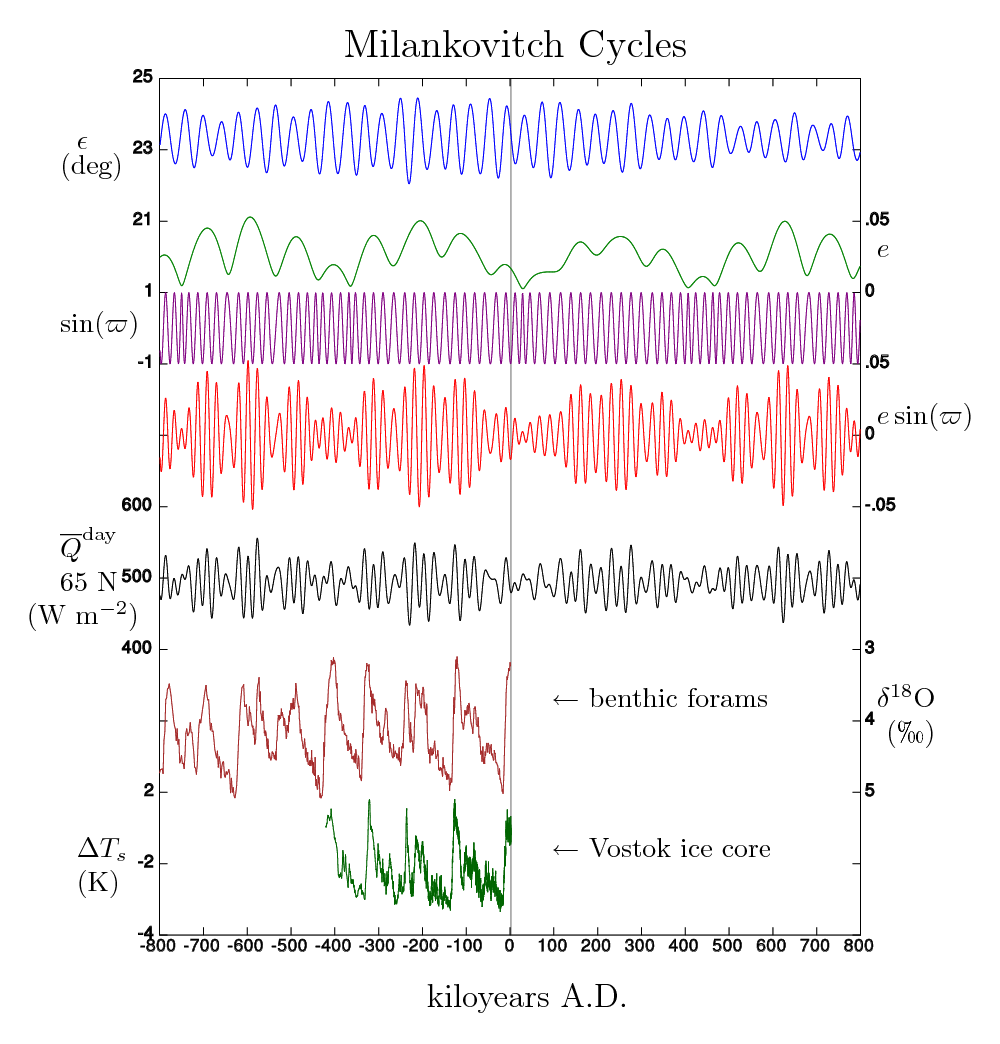
\includegraphics[width=6in]{milankovitch.png}
\end{center}

\newpage

\bigskip
\bigskip

\begin{center}
\Large Hints: Avoiding solar system drift
\end{center}

\normalsize

The total momentum of a system of two stars is

$$
\vec p =m_1 \vec v_1 + m_2 \vec v_2
$$

This gives a center-of-mass velocity of 

$$\vec v_{\rm com} = \frac{m_1 \vec v_1 + m_2 \vec v_2}{m_1+m_2}$$

By calculating this value and subtracting it from each of your objects' initial velocities,
you ensure that the total center-of-mass velocity (and thus the total momentum) is zero,
and your simulation won't drift. This can be done with code like the following:

\begin{verbatim}
double vxc,vyc; //center-of-mass velocities
vxc = (m1*vx1 + m2*vx2) / (m1+m2); 
vyc = (m1*vy1 + m2*vy2) / (m1+m2); 
vx1 = vx1 - vxc;
vy1 = vy1 - vyc;
vx2 = vx2 - vxc;
vy2 = vy2 - vyc;
\end{verbatim}

\end{document}

